\documentclass[a4paper,11pt]{article}
\usepackage{indentfirst}
\usepackage[T1]{fontenc}
\usepackage[polish]{babel}
\usepackage[utf8]{inputenc}
\usepackage{lmodern}
\selectlanguage{polish}
\usepackage[top=2cm, bottom=2cm, left=1cm, right=1cm]{geometry}
\usepackage{lastpage}
\usepackage{fancyhdr}
\pagestyle{fancy}
\setlength\parindent{24pt}
\makeatletter
\newcommand{\linia}{\rule{\linewidth}{0.4mm}}
\renewcommand{\maketitle}{\begin{titlepage}
    \vspace*{2cm}
    \begin{center}\LARGE
    Politechnika Warszawska\\
    Wydział Elektryczny\\
    \end{center}
    \vspace{5cm}
    \noindent\linia
    \begin{center}
      \LARGE \textsc{\@title}
         \end{center}
     \linia
    \vspace{0.5cm}
    \begin{flushright}
    \begin{minipage}{5cm}
    \textit{Autor:}\\
    \normalsize \textsc{\@author} \par
    \end{minipage}
    \vspace{5cm}
     \end{flushright}
    \vspace*{\stretch{6}}
    \begin{center}
    \@date
    \end{center}
  \end{titlepage}
}
\makeatother
\author{Grzegorz Kopyt \\ Arkadiusz Michalak}
\title{Specyfikacja Funkcjonalna\\Projekt Zespołowy 2018/2019}
\usepackage{graphicx}

\fancyhf{}
\rfoot{\thepage{}/\pageref{LastPage}}

\begin{document}
\maketitle

\tableofcontents
\vspace{1cm}
\noindent\linia
\section{Wstęp teoretyczny}
Dokument ten dotyczy programu realizowanego w ramach ,,Projektu Zespołowego 2018/2019".

Głównym zadaniem jest analiza i podział terenu na optymalne części. Program na podstawie podanego konturu terenu oraz punktów kluczowych, znajdujących się na tym terenie, powinien podzielić go na optymalne części. Oznacza to, że każdy z powstałych obszarów powinien zawierać jeden punkt kluczowy, a granice powinny obejmować każde miejsce, z którego bliżej jest do danego punktu kluczowego niż do jakiegokolwiek innego z~punktów kluczowych.

Dodatkowo na całą mapę zostaną naniesione różne typy obiektów (między innymi domy z mieszkańcami), a~program powinien przygotować statystykę ilości obiektów oraz mieszkańców na danej części terenu.

Ważnym założeniem jest to, że pod danymi współrzędnymi może znajdować się tylko jeden punkt kluczowy lub obiekt.

Pozostałe funkcje programu zostały opisane w sekcji ,,Wymagania funkcjonalne".

\noindent\linia
\section{Wymagania funkcjonalne}
\noindent
Program powinien spełniać podane wymagania funkcjonalne:
\begin{itemize}
\item podanie danych z pliku:
\begin{itemize}
\item podanie konturu terenu,
\item podanie z rozmieszczeniem punktów kluczowych,
\item podawanie obiektów i definiowanie ich typów.
\end{itemize}
\item analiza terenu:
\begin{itemize}
\item podzielenie terenu na optymalne obszary,
\item wyświetlanie listy obiektów należących do danego obszaru,
\item wyświetlanie zbiorcze listy obiektów należących do danego obszaru,
\item wyświetlanie liczby mieszkańców danego obszaru.
\end{itemize}
\item wizualizacja:
\begin{itemize}
\item narysowanie granic optymalnych obszarów,
\item naniesienie na wczytany teren obiektów.
\end{itemize}
\item modyfikacja po wprowadzeniu danych z pliku:
\begin{itemize}
\item dodawanie i usuwanie elementów konturu terenu,
\item dodawanie i usuwanie punktów kluczowych,
\item nakładanie grafiki pod wyznaczone kontury.
\end{itemize}
\end{itemize}

Plik wejściowy powinien być zgodny z podanym wzorem:

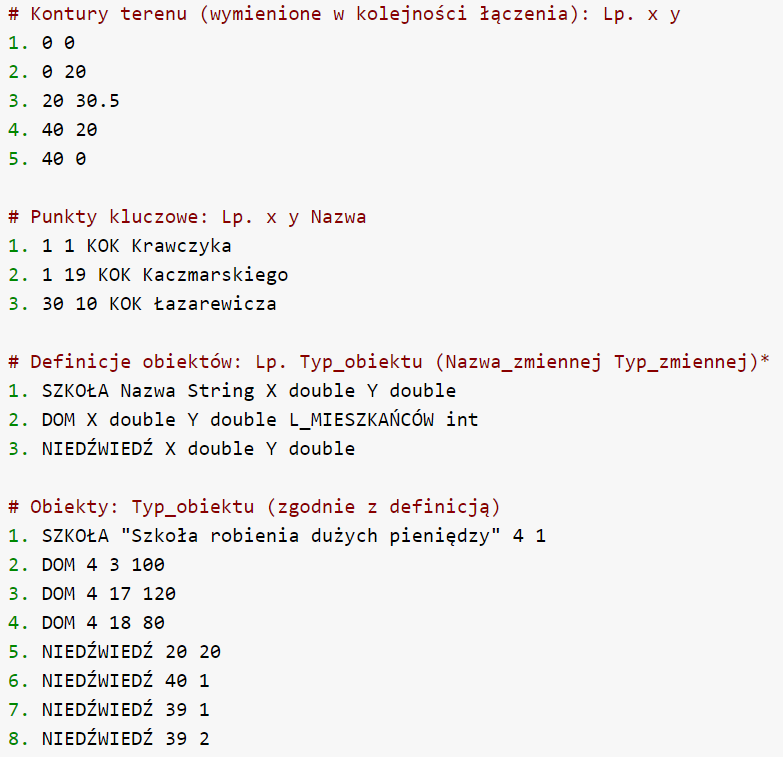
\includegraphics[scale=0.70]{ExampleInputFile}

\noindent
Uwagi:
\begin{itemize}
\item kolejne sekcje pliku powinny być oddzielane znakiem \textit{\#};
\item obsługiwane typy możliwe do użycia przy definicji nowych typów to: string, int, double;
\item wartości zmiennych typu string powinny być podane w cudzysłowie;
\item nazwy obiektów powinny być bez spacji i zawierać do 40 znaków;
\item podane punkty kluczowe i obiekty muszą znajdować się wewnątrz podanego konturu terenu lub na jego krawędzi;
\item jeśli podany kontur będzie otwarty, ostatni jego punkt zostanie połączony z pierwszym;
\item podany kontur musi być figurą wypukłą;
\item punkty konturu powodujące jego wklęsłość figury zostaną zignorowane;
\item kolejne punkty konturu muszą być podawane w kolejności łączenia;
\item punkty konturu powinny być podawane w kolejności zgodnej z ruchem wskazówek zegara;
\item krawędzie konturu terenu nie mogą się przecinać;
\item żadna współrzędna obiektu lub punktu kluczowego nie może się powtórzyć;
\item muszą zostać podane obiekty \textit{DOM}, \textit{NIEDŹWIEDŹ}, \textit{SZKOŁA} wraz z ich definicjami, takimi jak w pliku przykładowym;
\item plik musi być kodowany w UTF-8;
\item maksymalna możliwa wartość współrzędnych \textit{x} i \textit{y} to \textit{500.0}.
\end{itemize}
\noindent\linia
\section{Obsługa}
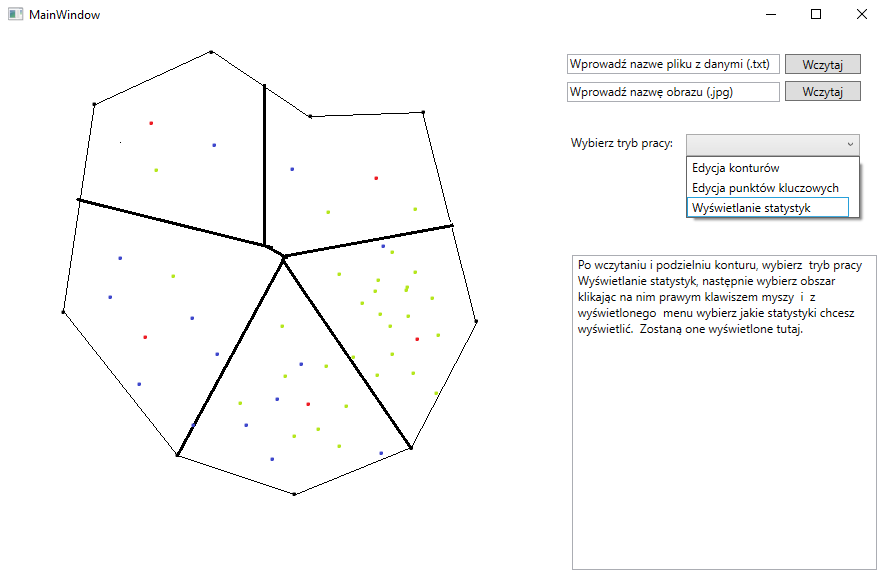
\includegraphics[scale=0.75]{GUI_EXAMPLE.png}

\noindent
Uruchomienie programu:
\begin{itemize}
\item po uruchomieniu programu należy wybrać plik danych. Po kliknięciu klawisza wyświetli się okno przeglądania plików, wzorzec pliku wejściowego znajduje się w \textbf{rozdziale 2};
\item opcjonalnie można wczytać obraz tła korzystając z odpowiedniego przycisku, wyświetla się okno przeglądania plików.
\end{itemize}
Tryb edycji konturów:
\begin{itemize}
\item po wybraniu tego trybu pracy użytkownik zyskuje możliwość zmiany wyglądu konturów analizowanego obszaru;
\item po wybraniu prawym przyciskiem myszy punktu konturu wyświetli się menu, punkt można usunąć, wtedy punty do niego sąsiednie zostaną połączone, można go również przesunąć zachowując obecne połączenie;
\item po wybraniu prawym przyciskiem linii konturu można dodać nowy punkt który zostanie połączony z punktami wyznaczającymi daną linie a~wybrana linia zostanie usunięta.
\end{itemize}
Tryb edycji punktów kluczowych:
\begin{itemize}
\item po wybraniu tego trybu pracy użytkownik może manipulować punktami kluczowym;
\item po wybraniu punktu prawym przyciskiem myszy wyświetli się menu, plik można usunąć lub przenieść go w inne miejsce;
\item w dowolnym pustym miejscu w konturze po kliknięciu prawym przyciskiem myszy pojawi się możliwość dodania nowego punktu kluczowego.
\end{itemize}

Tryb wyświetlania statystyk:
\begin{itemize}
\item sposób działania najważniejszego dla użytkownika trybu zostanie zawarty w interfejsie graficznym programu;
\item po wybraniu obszaru prawym przyciskiem myszy menu pozwoli określić jakie statystyki użytkownik chce wyświetlić w przygotowanym do tego oknie:
\begin{itemize}
\item lista obiektów należących do obszaru;
\item pogrupowana typami lista obiektów;
\item liczba mieszkańców danego obszaru.
\end{itemize}
\end{itemize}
\noindent\linia
\section{Komunikaty o błędach}
W przypadku wystąpienia błędu pojawi się okno z komunikatem o tym błędzie.

\noindent
Przykładowe komunikaty wyglądają następująco:
\begin{itemize}
\item nie podano pliku wejściowego:

\textit{Nie podano pliku.}
\item podano błędny plik wejściowy:

\textit{Nieprawidłowy plik. Linia 24 jest błędna. Porównaj ją z plikiem wzorcowym.}
\item podany plik nie jest kodowany w UTF-8:

\textit{Nieprawidłowy plik. Plik nie jest kodowany w UTF-8.}
\item podany kontur nie jest figurą wypukłą:

\textit{Zignorowano (1,2), (23,45), (15,34). Podany kontur terenu nie był figurą wypukłą.}
\item podane krawędzie konturu przecinają się:

\textit{Nieprawidłowy plik. Krawędzie konturu przecinają się.}
\item podany punkt kluczowy nie zawiera się wewnątrz konturu:

\textit{Zignorowano punkt kluczowy (3,5). Podany punkt nie zawiera się wewnątrz granic konturu.}
\item podany obiekt nie zawiera się wewnątrz konturu:

\textit{Zignorowano DOM (5,71). Podany obiekt nie zawiera się wewnątrz granic konturu.}
\item podany obiekt duplikuje współrzędne innego obiektu lub punktu kluczowego:

\textit{Zignorowano DOM (2,39). Podany obiekt duplikuje współrzędne innego obiektu lub punktu kluczowego.}
\item podany punkt kluczowy duplikuje współrzędne innego obiektu lub punktu kluczowego:

\textit{Zignorowano punkt kluczowy (2,39).  Podany punkt kluczowy duplikuje współrzędne innego obiektu lub punktu kluczowego.}

\end{itemize}

\noindent\linia
\section{Testy akceptacyjne}
\begin{itemize}
\item Odczyt pliku:
\begin{itemize}
\item wczytanie pliku zawierającego prosty kontur i kilka punktów kluczowych;
\item wczytanie pliku z konturem, którego krawędzie przecinają się;
\item wczytanie pliku z punktami, których współrzędne są takie same jak innego punktu lub obiektu;
\item wczytanie pliku z obiektami, których współrzędne są takie same jak innego punktu lub obiektu;
\item wczytanie pliku z nieprawidłową definicją typu;
\item wczytanie pliku bez punktów kluczowych;
\item wczytanie pliku bez konturu;
\item wczytanie pliku z prawidłowymi danymi;
\item wczytanie pliku z obiektem poza granicami konturu;
\item wczytanie pliku z punktem kluczowym poza granicami konturu;
\item wczytanie pliku z konturem, który nie jest figurą wypukłą;
\item wczytanie pliku z konturem, którego punkt początkowy nie łączy się krawędzią z końcowym.
\end{itemize}
\item Modyfikacja:
\begin{itemize}
\item dodanie nowego punktu kluczowego w obszarze konturu;
\item próba dodania punktu kluczowego poza obszarem konturu;
\item próba dodania punktu kluczowego nad innym obiektem;
\item przesunięcie punktu wyznaczającego kontur w taki sposób, że krawędzie będą się przecinać;
\item przesunięcie punktu wyznaczającego kontur w taki sposób, że kontur nie będzie figurą wypukłą;
\item dodanie grafiki tła o dużej rozdzielczości;
\item dodanie grafiki tła niskiej rozdzielczości.
\end{itemize}
\item{Wyświetlanie statystyk:}
\begin{itemize}
\item sprawdzenie liczby mieszkańców dowolnego obszaru;
\item sprawdzenie liczby mieszkańców obszaru na którym nie ma mieszkańców;
\item wyświetlenie wszystkich obiektów obszaru na którym znajduje się około 100 obiektów;
\item wyświetlenie pogrupowanych obiektów obszaru;
\item wyświetlenie obiektów obszaru który nie ma obiektów.
\end{itemize}

\end{itemize}
Program będzie uznany za działający jeśli pozytywnie przejdzie wszystkie testy. Pod słowem pozytywnie rozumie się wyświetlenie rezultatów, lub odpowiedni komunikat błędu który pozwoli użytkownikowi naprawić błąd. W dziale statystyki szczególnie ważna jest przejrzystość wyświetlanych danych.

\noindent\linia

\end{document}



